%!TEX root = ../tesis_mbc.tex

\chapter{Resultados}

Los algoritmos presentados en este trabajo fueron implementados en el lenguaje para cómputo estadístico R y fueron probados con un conjunto de películas calificadas de \textit{MovieLens}, una página que ofrece recomendaciones de películas, los cuales están disponibles al público. \textit{MovieLens} es un proyecto de \textit{GroupLens}, un equipo de investigación de la Universidad de Minnesota orientado al cómputo social.

\subsection{Análisis exploratorio de datos}

\subsubsection{\textit{MovieLens}}

El conjunto de datos de \textit{MovieLens} consiste en \numprint{20000263} calificaciones de \numprint{26744} películas hechas por \numprint{138493} usuarios. Todos los usuarios habían calificado al menos 20 películas. Las calificaciones están en una escala de $0.5$ a $5$, con intervalos de medio punto, es decir, se puede poner $0.5, 1, \hdots, 4.5, 5$ como calificación \cite{harper2016movielens}. La distribución de las calificaciones se puede ver en la figura \ref{fig:ML_frec_calificaciones}; mientras que en la figura \ref{fig:ML_hist_prom_cals} se puede ver el histograma de los promedios por película.

\begin{figure}
	\centering
 	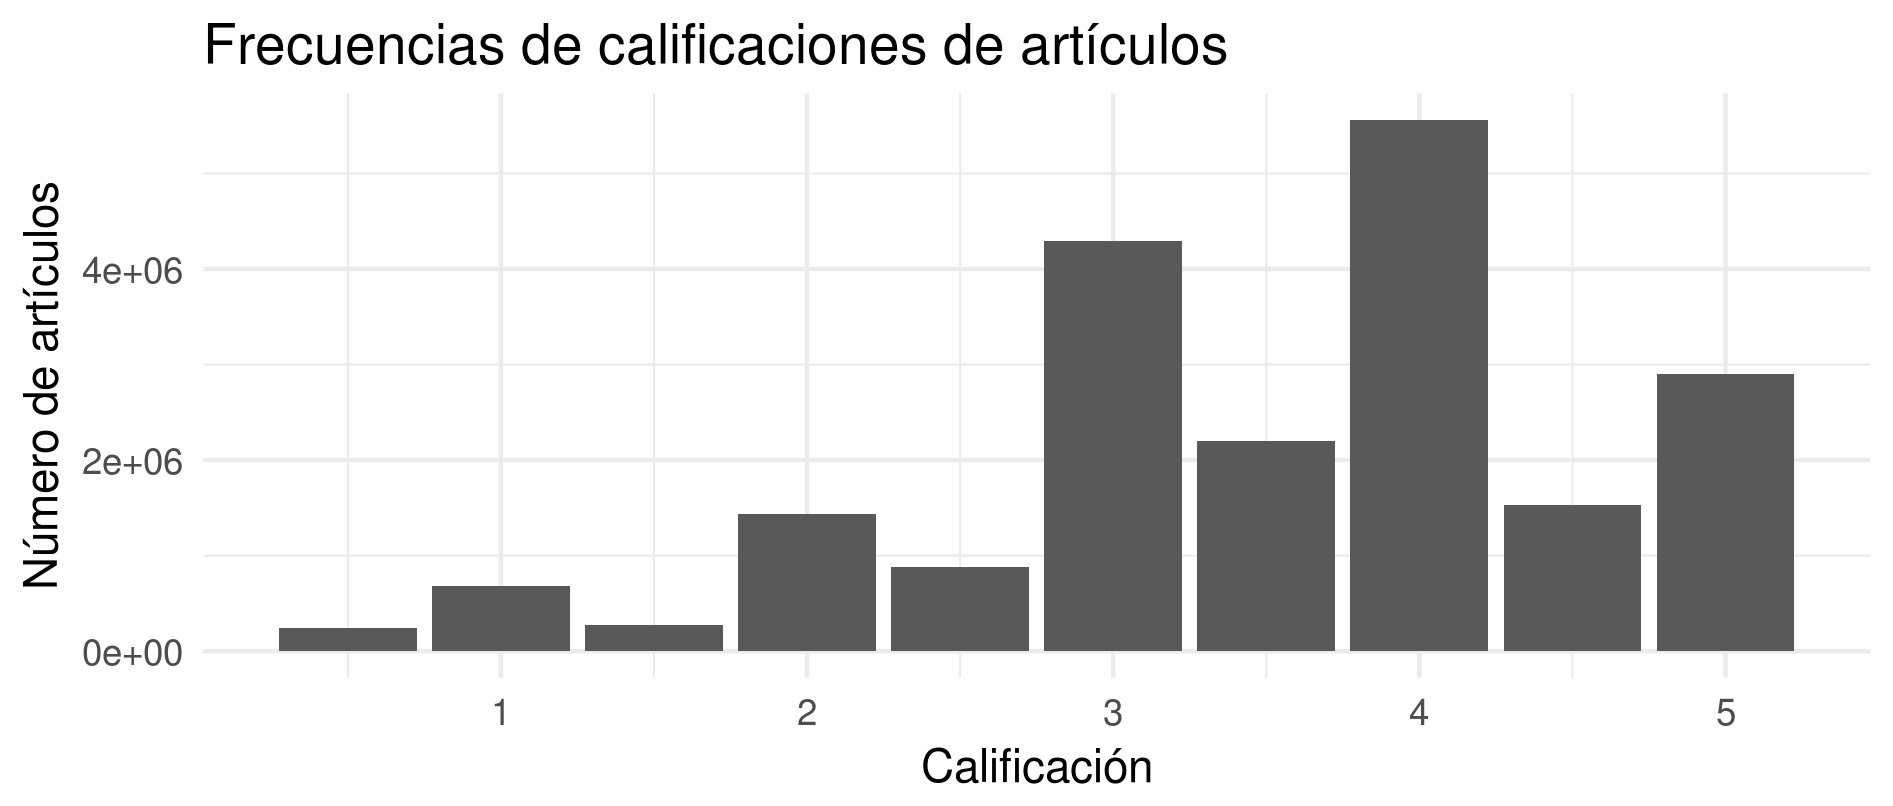
\includegraphics[width=0.9\textwidth]{frecuencia_calificaciones_MovieLens.png}
 	\caption{Frecuencia de calificaciones del conjunto de datos \textit{MovieLens}.}
 	\label{fig:ML_frec_calificaciones}
\end{figure}

\begin{figure}
	\centering
 	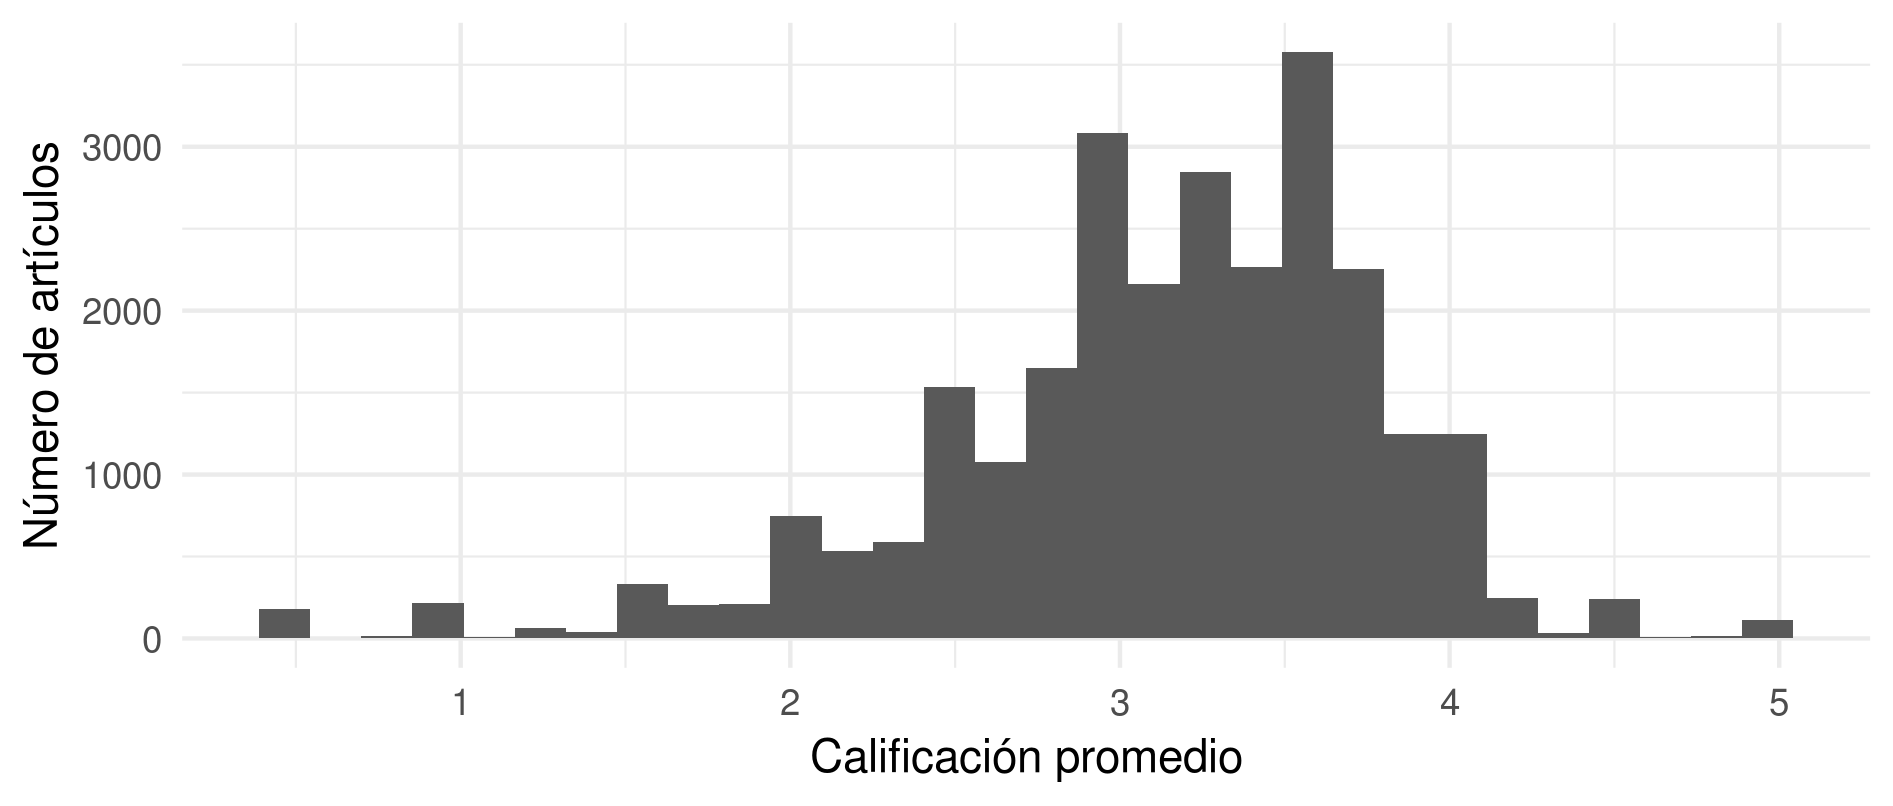
\includegraphics[width=0.9\textwidth]{calificacion_promedio_articulo_MovieLens.png}
 	\caption{Histograma del promedio de calificaciones por película del conjunto de datos \textit{MovieLens}.}
 	\label{fig:ML_hist_prom_cals}
\end{figure}

En la sección \ref{motivacion} se introduce el concepto de cola larga. En la figura \ref{fig:ML_long_tail} se puede ver cómo este fenómeno ocurre en los datos de \textit{MovieLens}, donde es claro que muy pocas películas tienen una gran cantidad de calificaciones, mientras que muchos artículos tienen pocas calificaciones.

\begin{figure}
	\centering
 	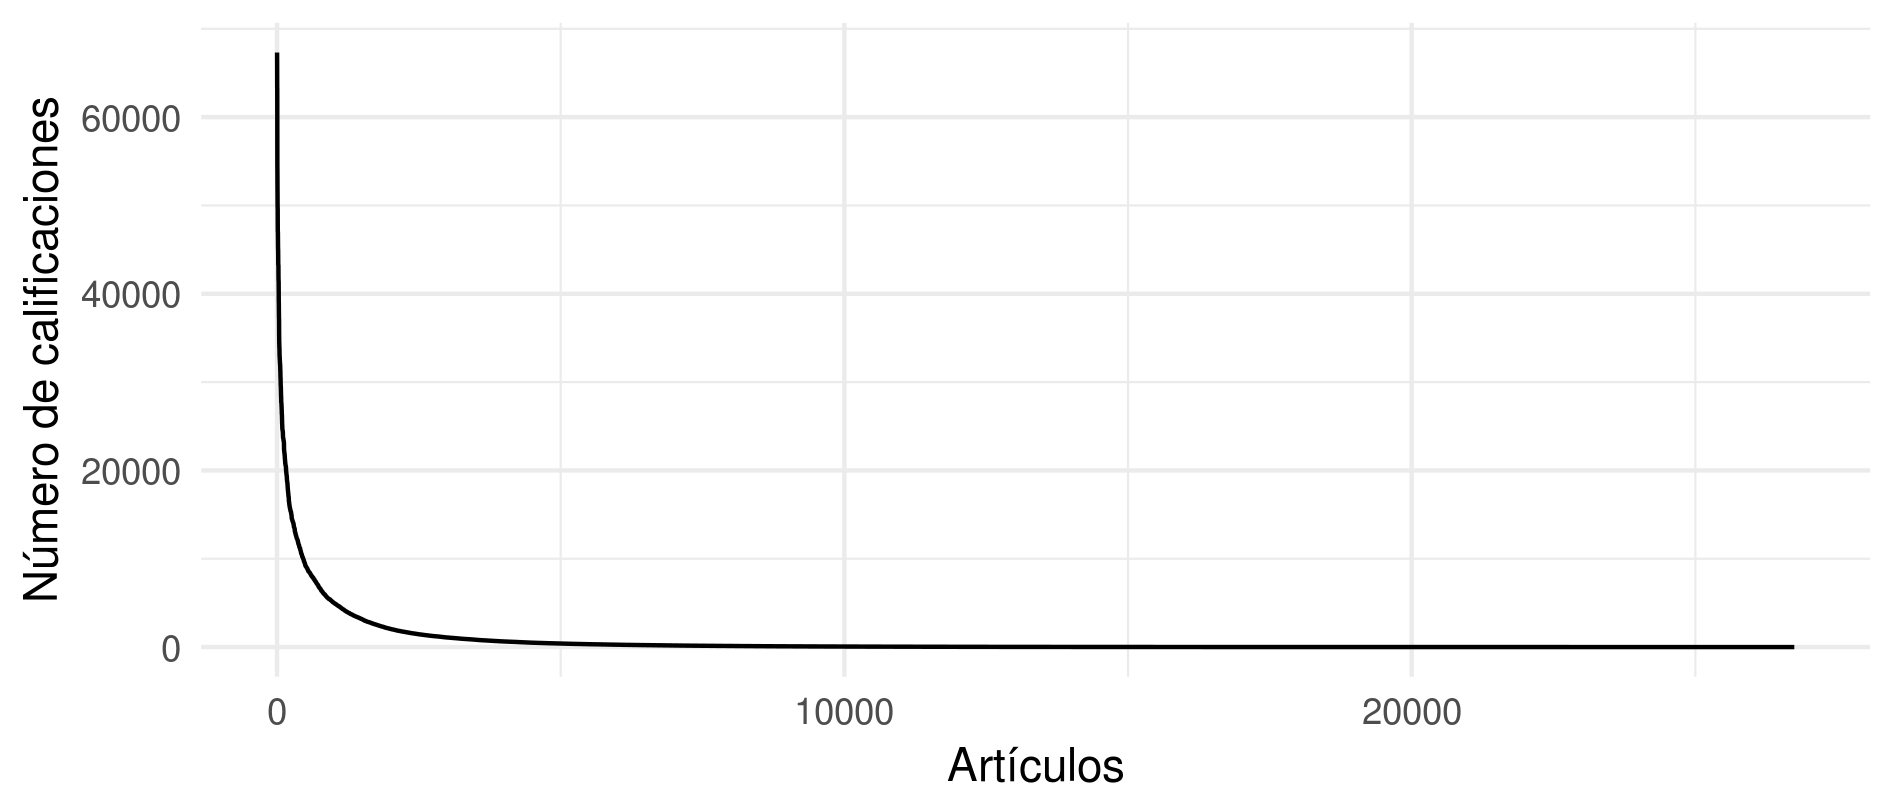
\includegraphics[width=0.9\textwidth]{long_tail_MovieLens.png}
 	\caption{Cola larga del conjunto de datos \textit{MovieLens}.}
 	\label{fig:ML_long_tail}
\end{figure}








\subsubsection{\textit{BookCrossing}}

El conjunto de datos de \textit{BookCrossing} consiste en \numprint{1149780} calificaciones de \numprint{271379} libros hechas por \numprint{278858} usuarios. Los datos se obtuvieron durante cuatro semanas de agosto a septiembre de 2004. Las calificaciones están en una escala de $1$ a $10$, con intervalos de un punto, es decir, se puede poner $1, 2, \hdots, 9, 10$ como calificación. Se tiene como calificación especial el $0$, el cual es solamente una calificación implícita, es decir, si leyó o no el libro \cite{ziegler2005improving}. Debido a que para usar el método presentado en este trabajo se necesitan calificaciones explícitas, se filtraron estas del conjunto de datos original. Con esta operación, quedaron \numprint{383852} calificaciones de \numprint{153683} libros hechas por \numprint{68092} usuarios. La distribución de las calificaciones filtradas se puede ver en la figura \ref{fig:BC_frec_calificaciones}; mientras que en la figura \ref{fig:BC_hist_prom_cals} se puede ver el histograma de los promedios por libro.

\begin{figure}
	\centering
 	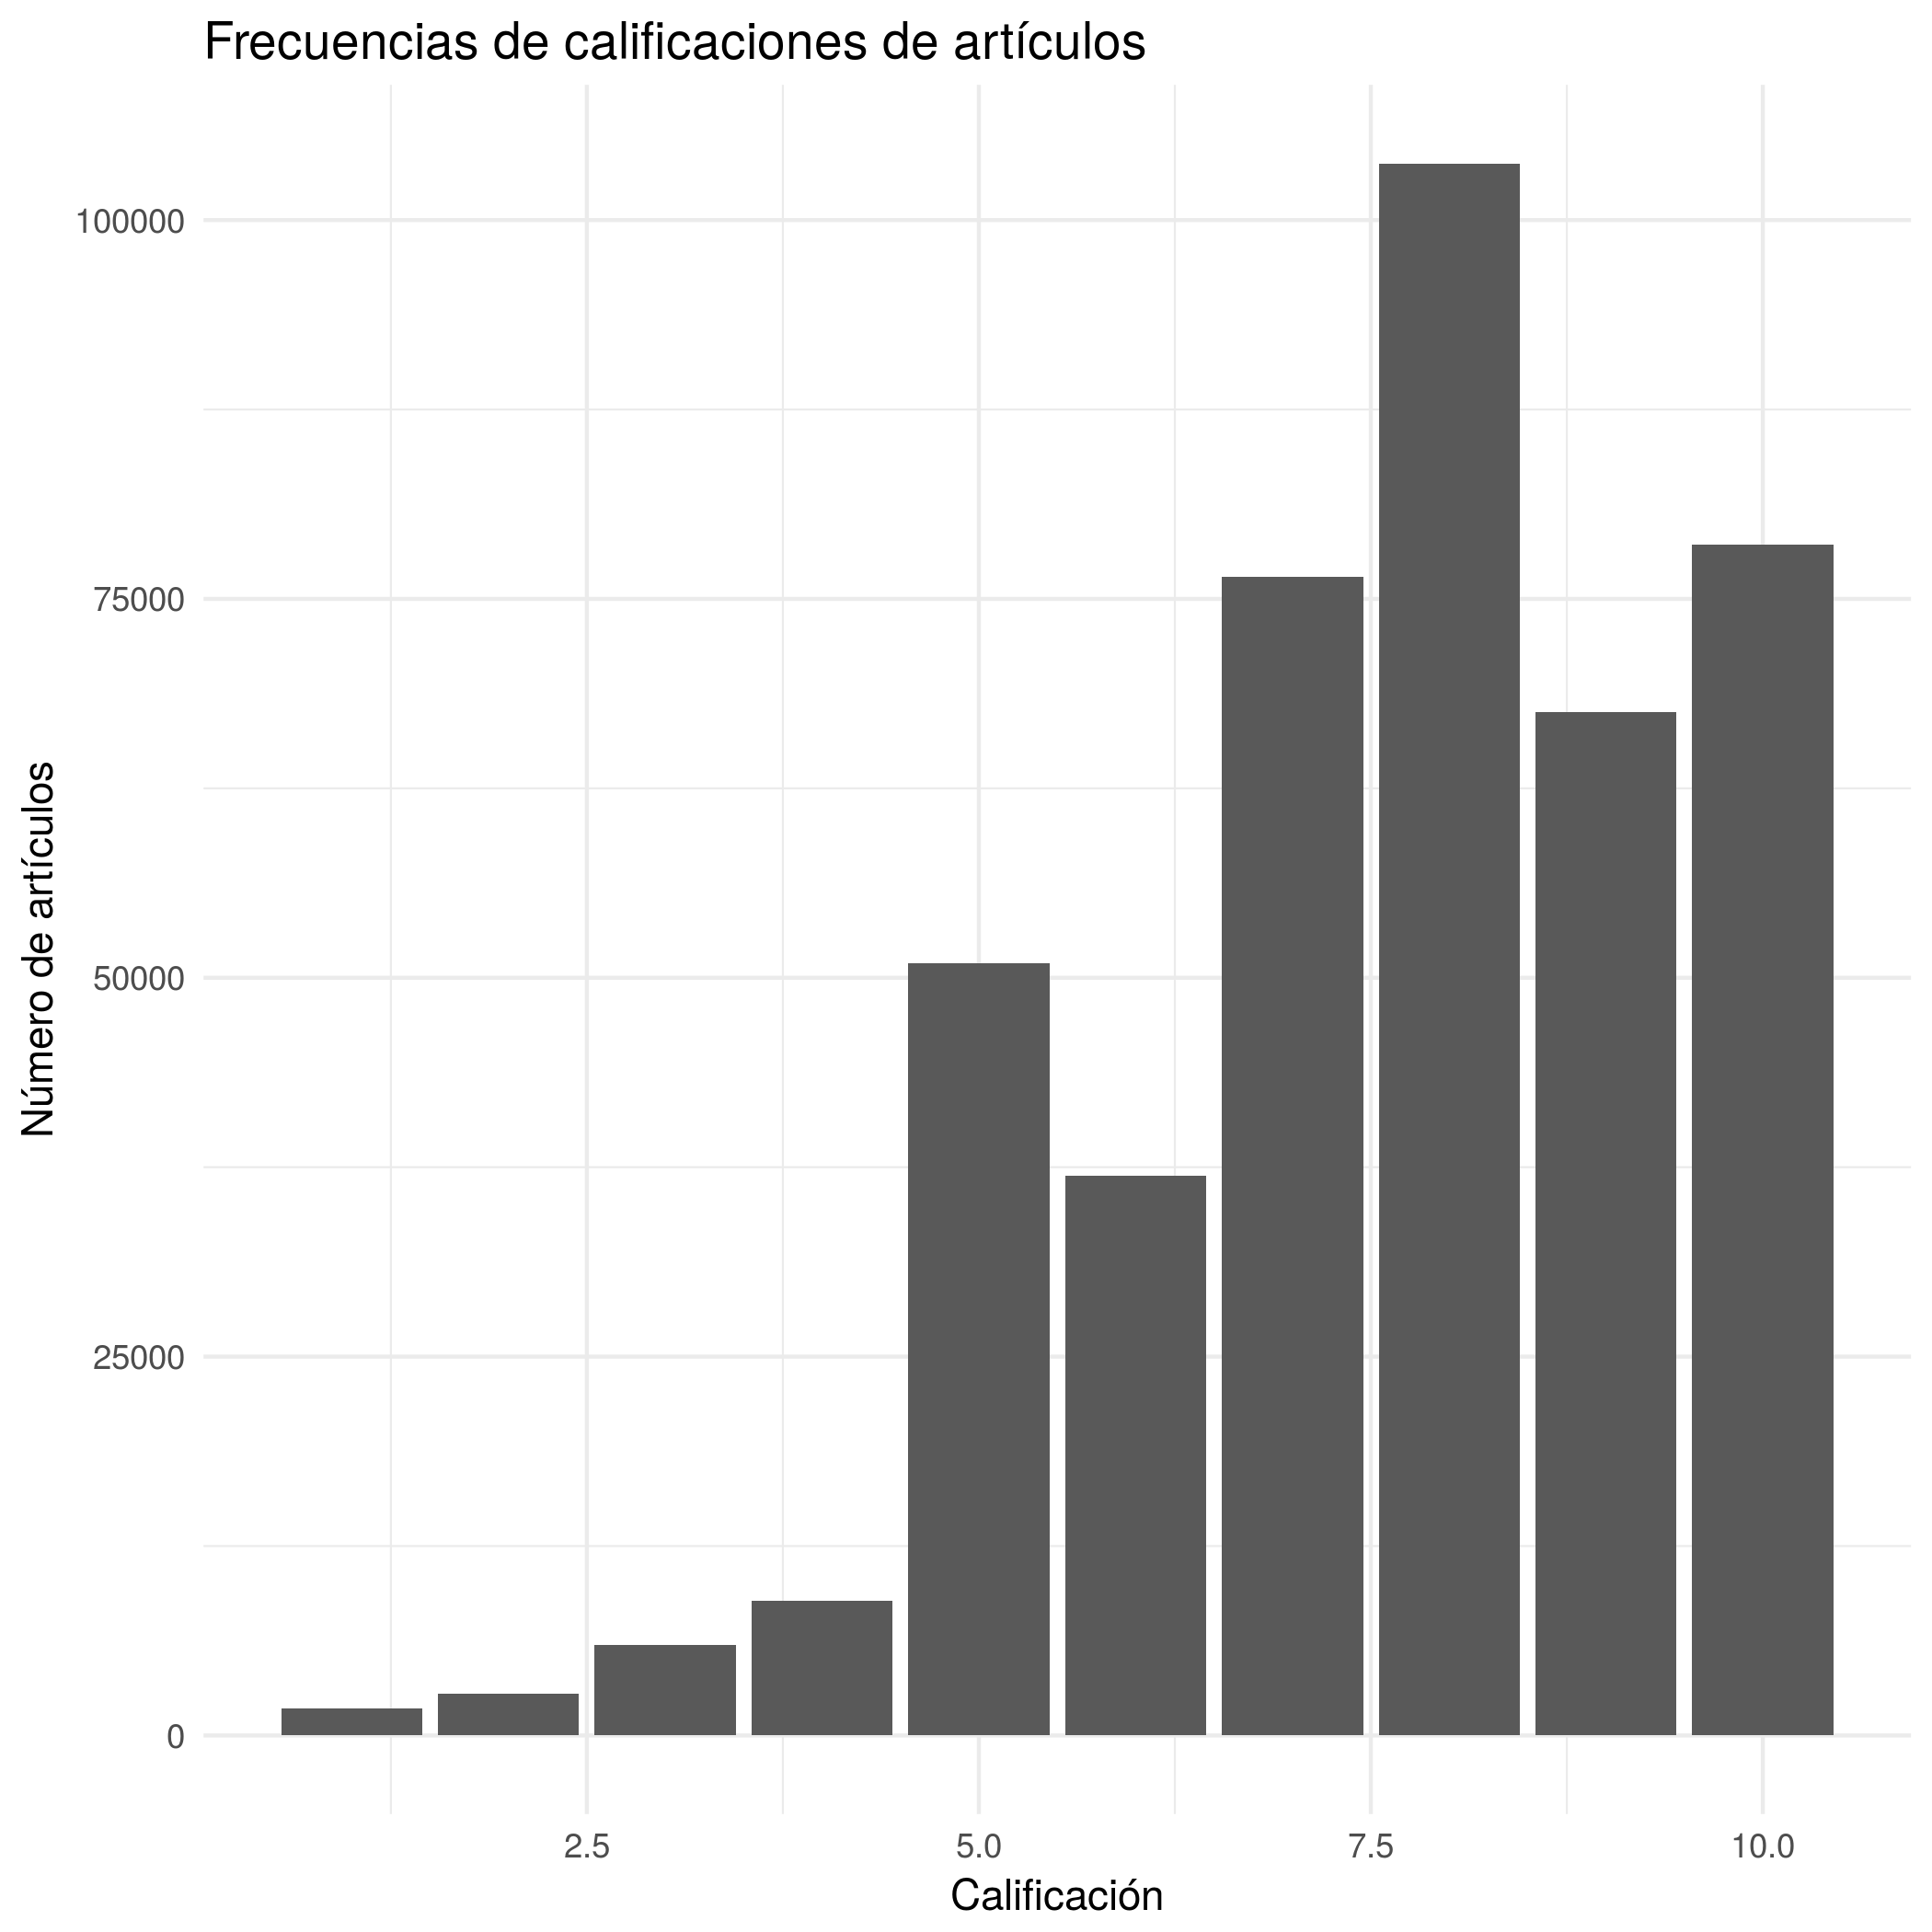
\includegraphics[width=0.9\textwidth]{frecuencia_calificaciones_BookCrossing.png}
 	\caption{Frecuencia de calificaciones del conjunto de datos \textit{BookCrossing}.}
 	\label{fig:BC_frec_calificaciones}
\end{figure}

\begin{figure}
	\centering
 	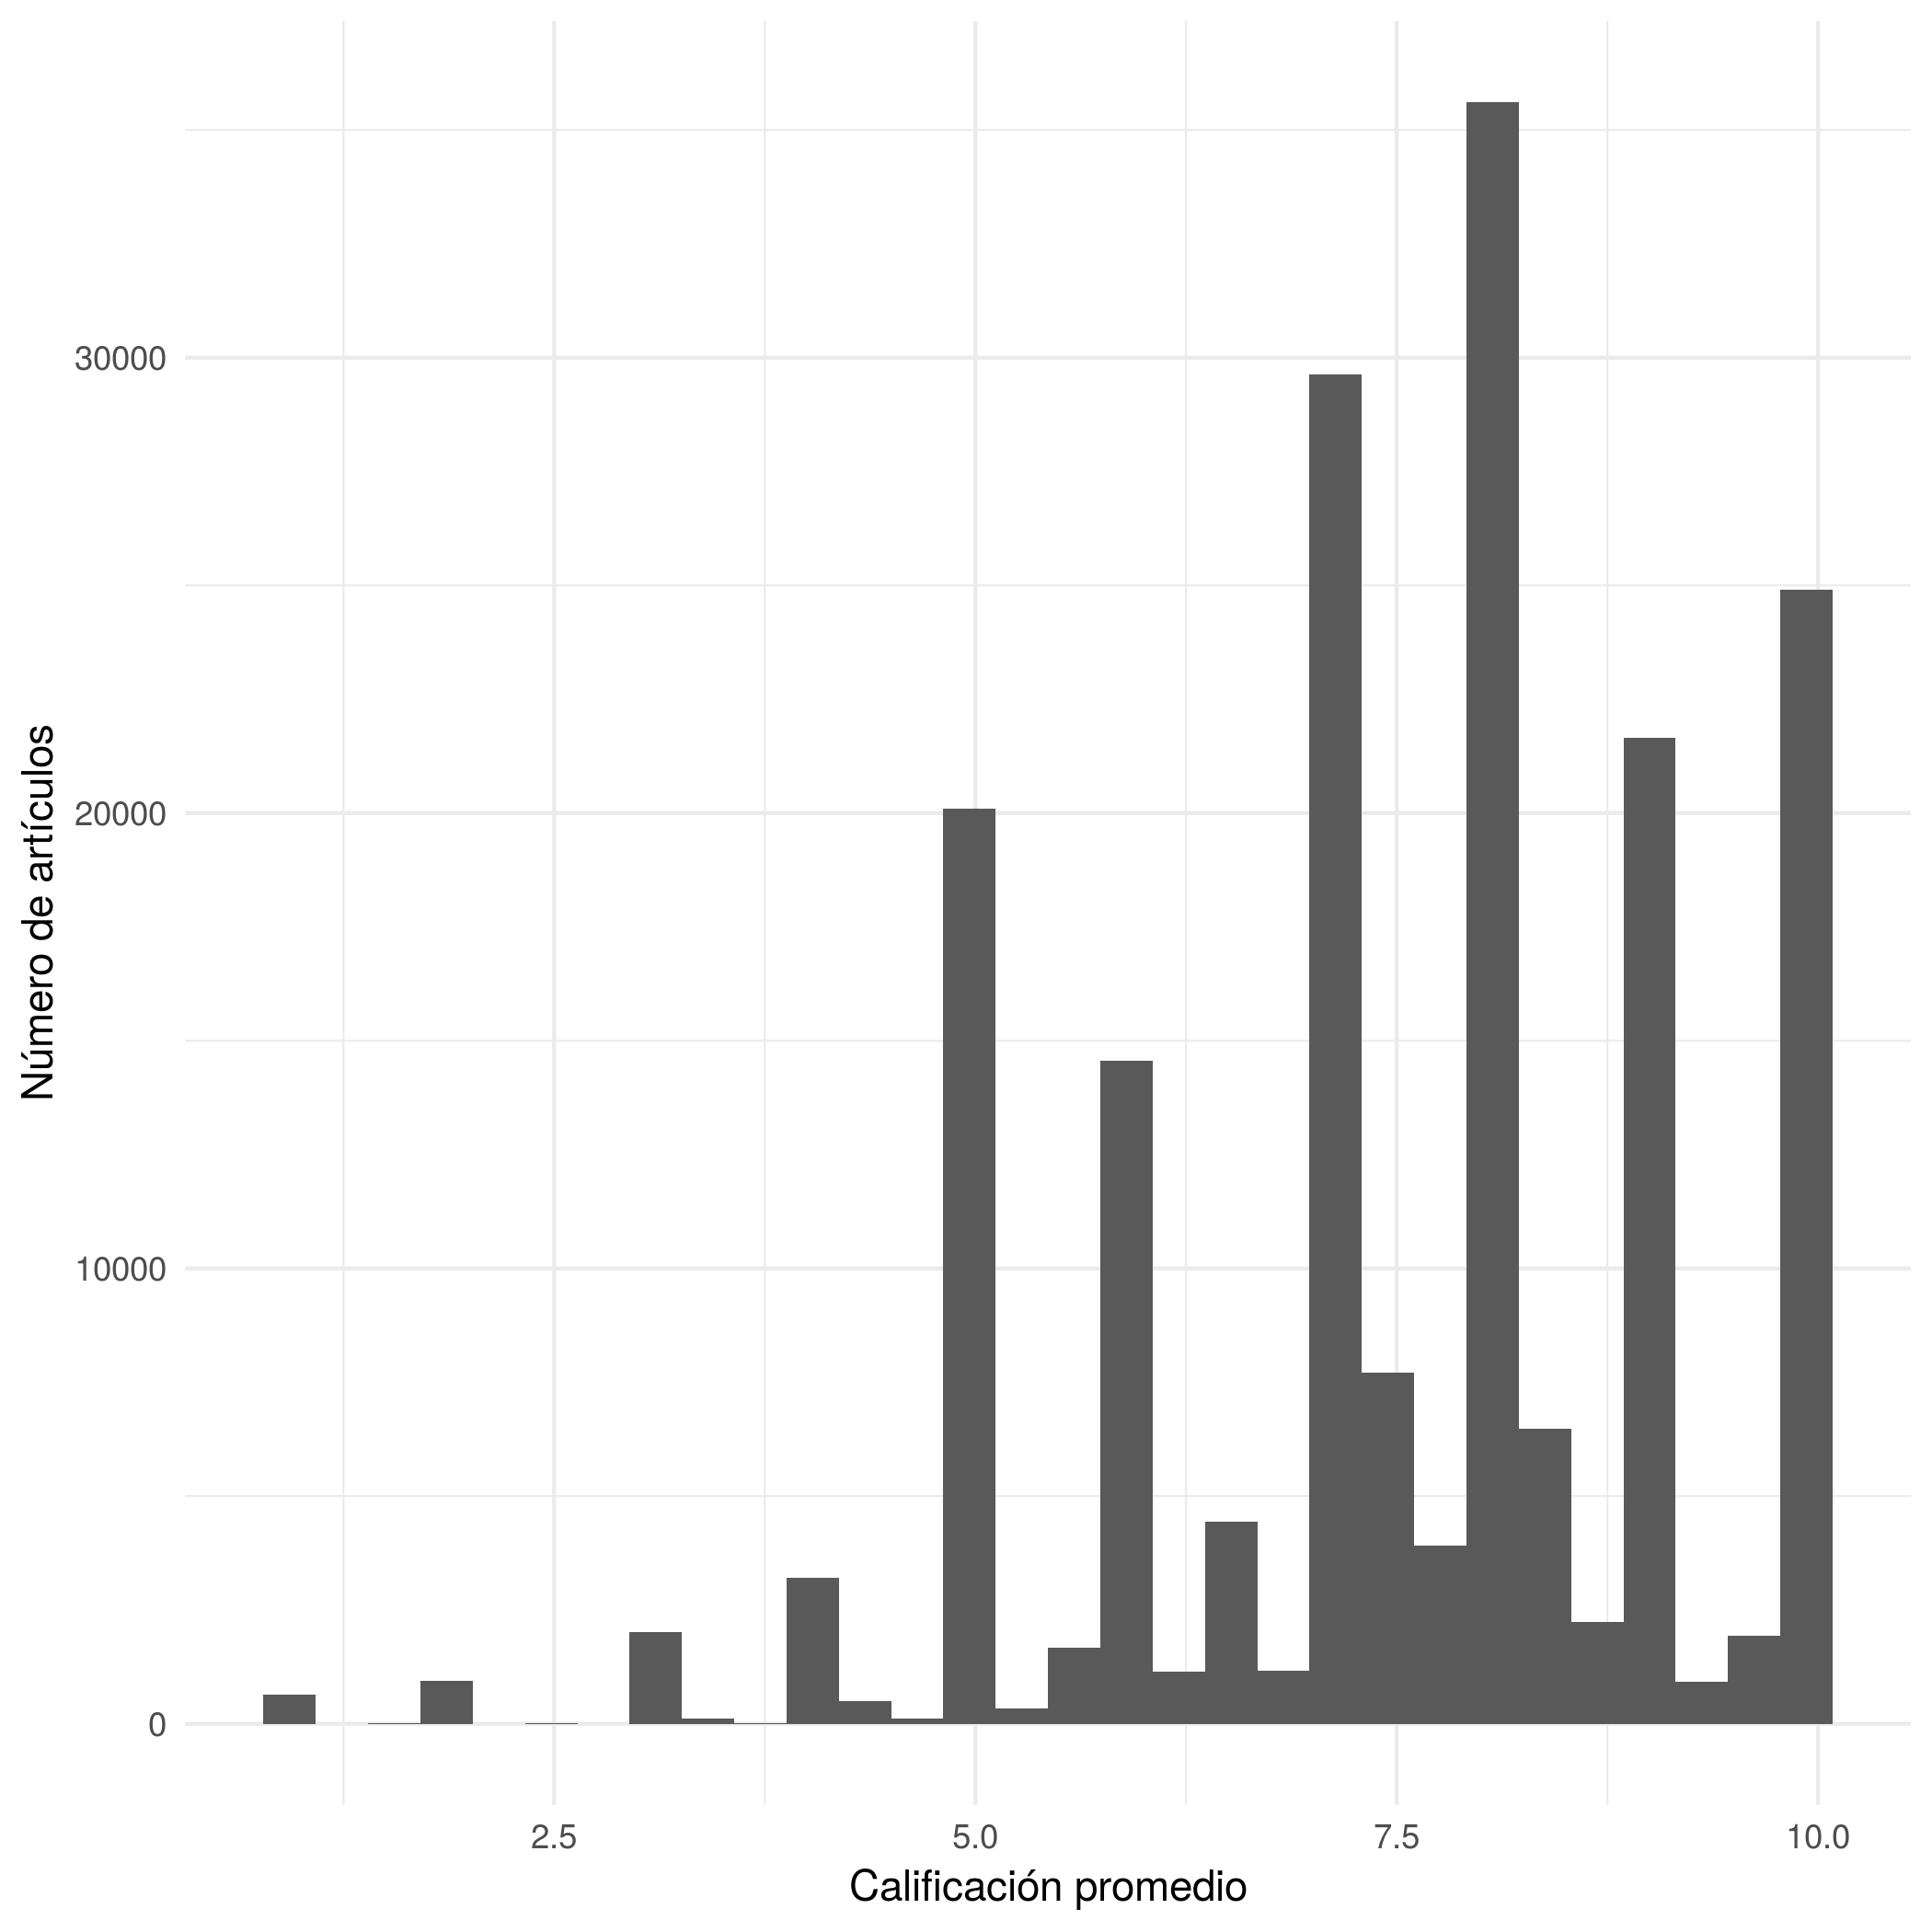
\includegraphics[width=0.9\textwidth]{calificacion_promedio_articulo_BookCrossing.png}
 	\caption{Histograma del promedio de calificaciones por película del conjunto de datos \textit{BookCrossing}.}
 	\label{fig:BC_hist_prom_cals}
\end{figure}

En la figura \ref{fig:BC_long_tail} se puede ver la cola larga en los datos de \textit{BookCrossing}, donde nuevamente es claro que muy pocas películas tienen una gran cantidad de calificaciones, mientras que muchos artículos tienen pocas calificaciones.

\begin{figure}
	\centering
 	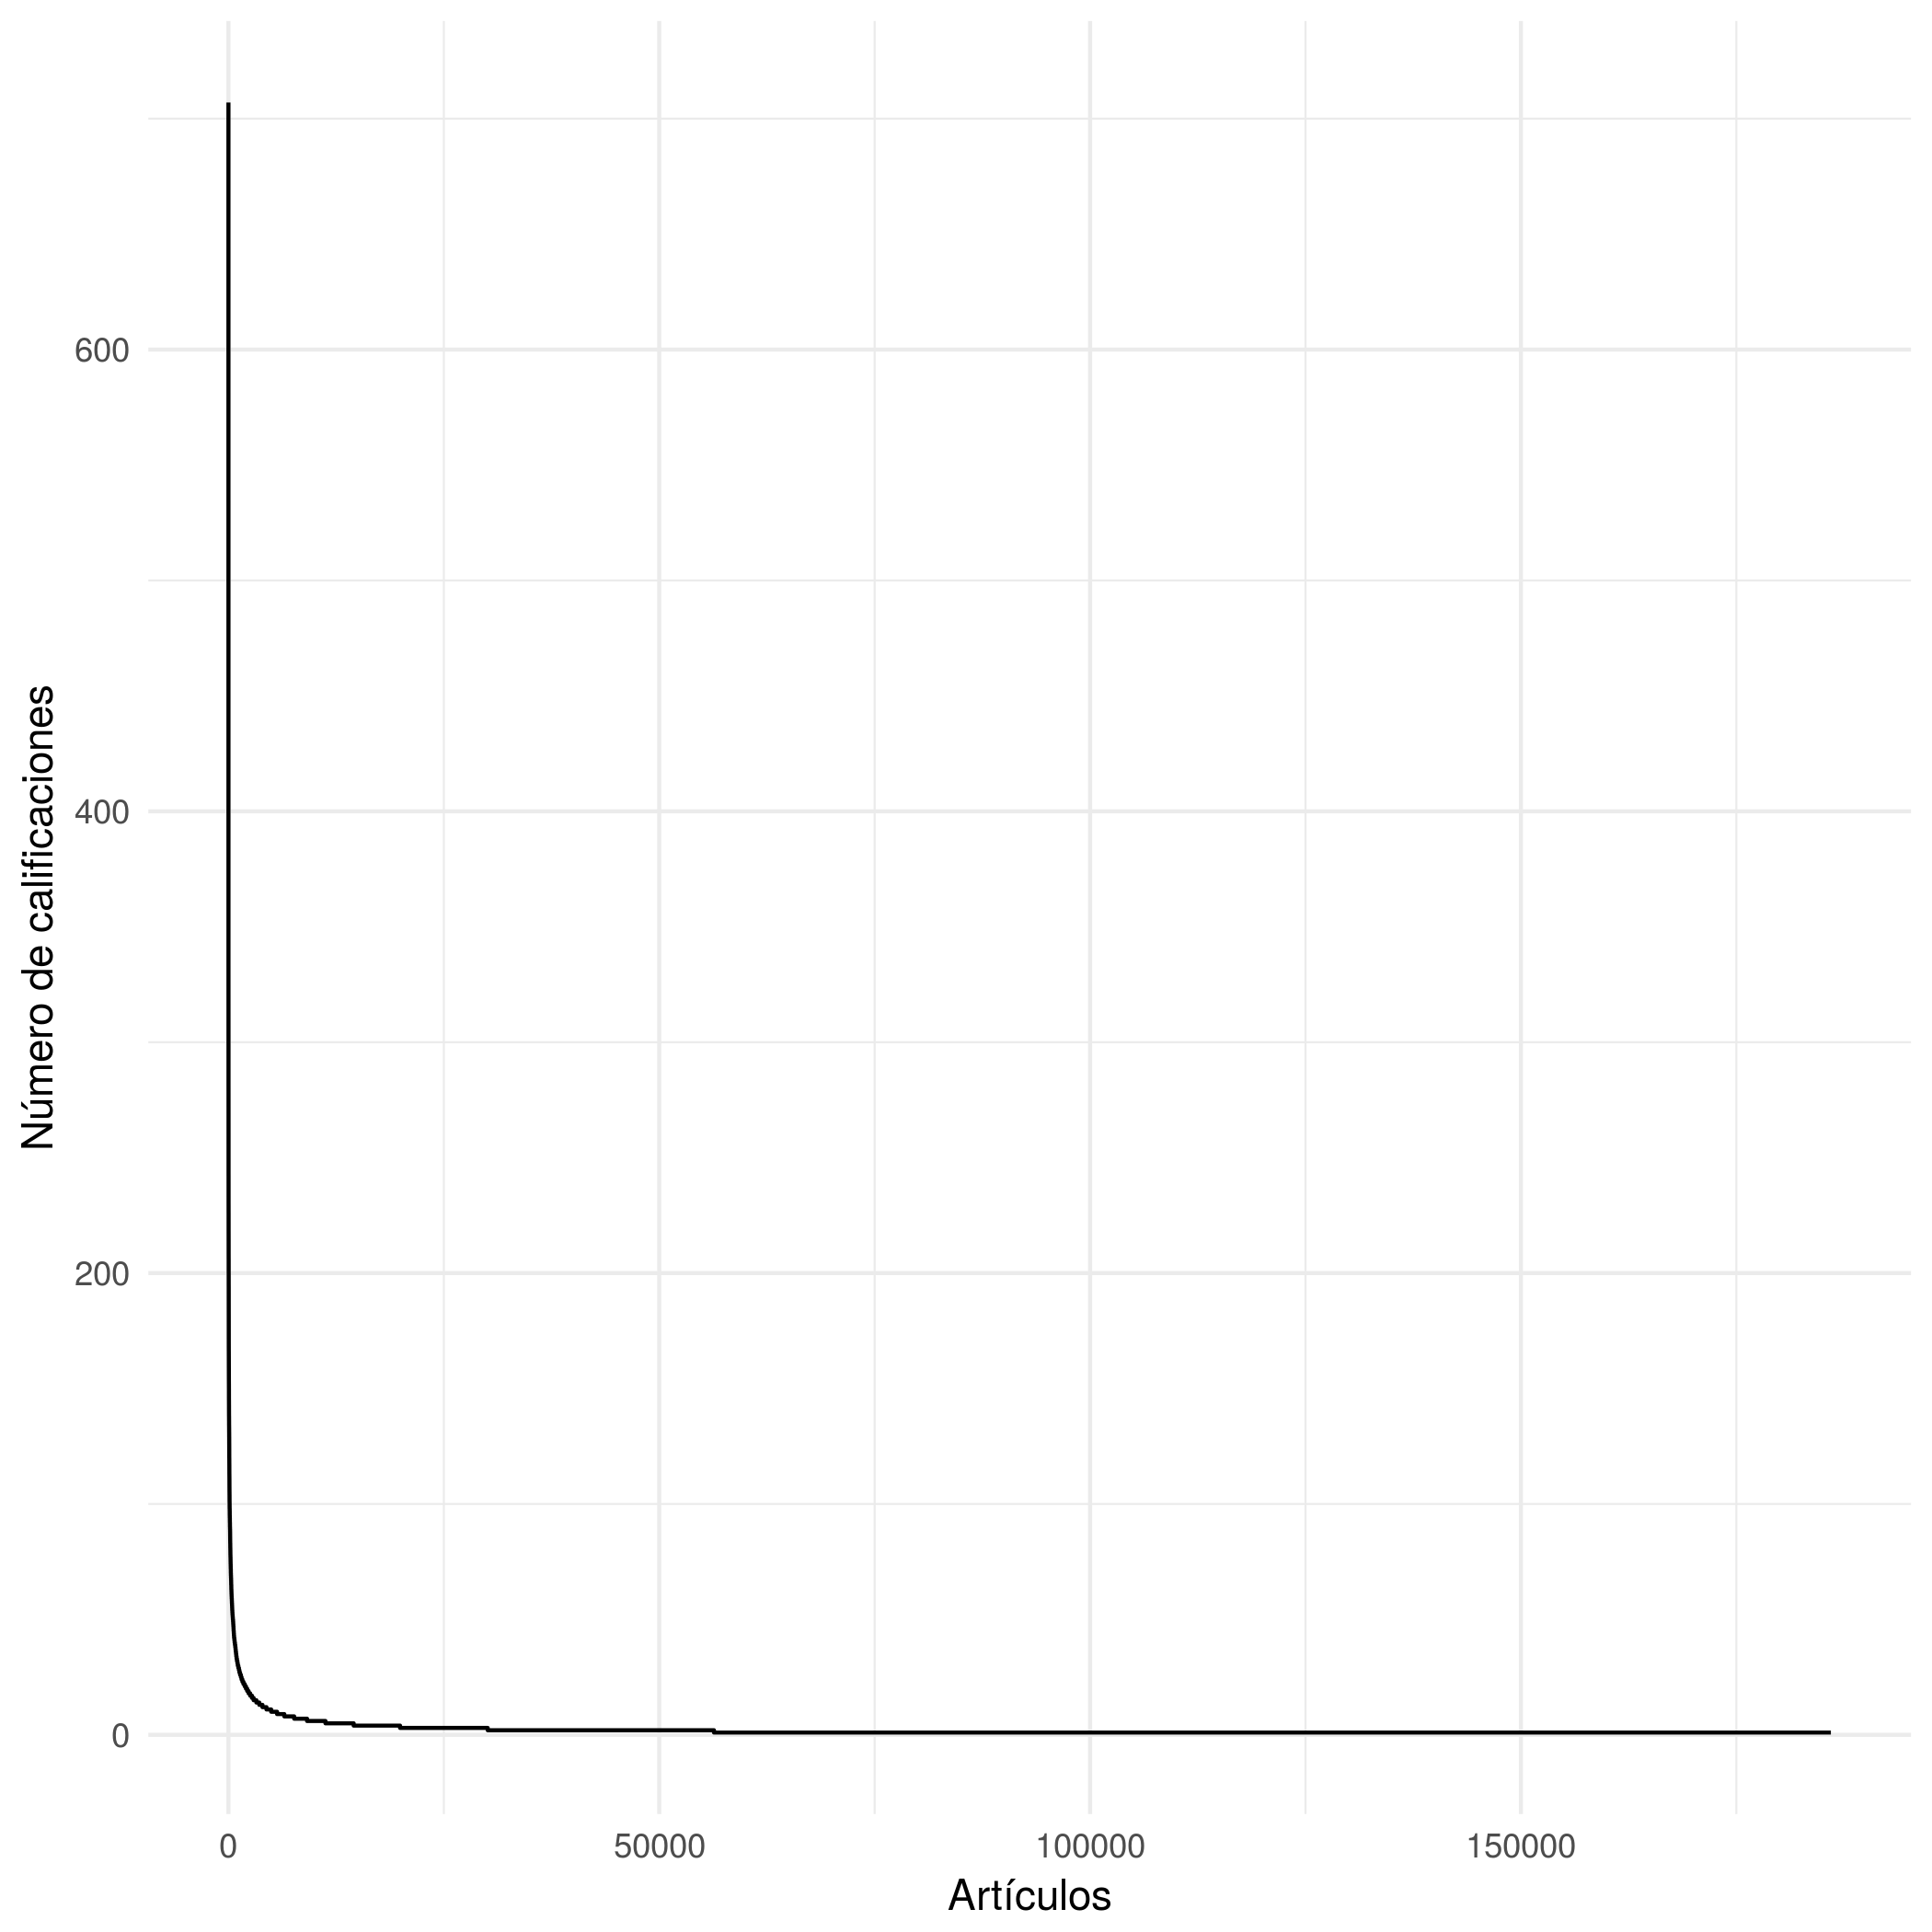
\includegraphics[width=0.9\textwidth]{long_tail_BookCrossing.png}
 	\caption{Cola larga del conjunto de datos \textit{BookCrossing}.}
 	\label{fig:BC_long_tail}
\end{figure}